\input ../preamble

\begin{document}

{\Huge

  \centerline{\bf TTIC 31230, Fundamentals of Deep Learning}
  \bigskip
  \centerline{David McAllester, April 2017}
\vfill
  \centerline{\bf Deep Reinforcement Learning}
  \vfill
\vfill

\slide{Definition of Reinforcement Learning}

RL is defined by the following properties:

\vfill
\begin{itemize}
\item An environment with {\bf state}.

  \vfill
\item State changes are influenced by {\bf sequential decisions}.

  \vfill
\item  Reward (or loss) depends on {\bf making decisions} that lead to {\bf desirable states}.
\end{itemize}

\slide{Reinforcement Learning Examples}

\begin{itemize}
\item Board games (chess or go)

  \vfill
\item Atari Games (pong)

  \vfill
\item Robot control (driving)

  \vfill
\item Dialog

  \vfill
\item Life

\end{itemize}

\slide{Policies}

A policy is a way of behaving.

\vfill
Formally, a (nondeterministic) policy maps a state to a probability distribution over actions.

\vfill
\begin{eqnarray*}
    \pi(a_t|s_t) & & \mbox{probability of action $a_t$ in state $s_t$}
\end{eqnarray*}

\slide{Imitation Learning}

Construct a training set of state-action pairs $(s,a)$ from experts.

\vfill
Define stochastic policy $\pi_\Theta(s)$.

\vfill
$$\Theta^* = \argmin_\Theta \expectsub{(s,a) \sim \mathrm{Train}}{- \ln \pi_\Theta(a\;|\;s)}$$

\vfill
This is just cross-entropy loss.

\slide{Dangers of Imperfect Imitation Learning}

Perfect imitation learning would reproduce expert behavior.

Imitation learning is {\bf off-policy} ---
the state distribution in the training data is different from that defined by the policy being learned.

\vfill
Imitating experts can be dangersous.  ``Don't try this at home''.

\vfill
Also, imitating experts will never exceed expert performance (consider AlphaZero).

\slide{Markov Decision Processes (MDPs)}

For an RL problem we work with an action policy $\pi$

\vfill
$s_t$ is the state at time $t$

\vfill
$r_t$ is the reward at time $t$

\vfill
$a_t$ is the action taken at time $t$.
\begin{eqnarray*}
  r_t = R(s_t,a_t) & & \mbox{reward at time $t$} \\
  \\
  T(s_{t+1}|s_t,a_t) & & \mbox{state transition probability}
\end{eqnarray*}

\vfill
The state space, action space, $R$ and $T$ define a {\bf Markov Decision Process} or {\bf MDP}.

\slide{Optimizing Reward}

In RL we maximize reward rather than minimize loss.

$$\pi^* = \argmax_\pi \;R(\pi)$$

\vfill
$$\begin{array}{rcll}
  R(\pi) & = & \expect{\sum_{t=0}^T \;r_t} &\mbox{episodic reward (go)} \\
\\
& \mbox{or} & \expect{\sum_{t=0}^\infty \;\gamma^t r_t} &\mbox{discounted reward} \\
\\
& \mbox{or} & \lim_{T \rightarrow \infty}\;\frac{1}{T} \;\sum_{t=0}^T \;r_t &\mbox{asymptotic average reward (driving)}
\end{array}$$


\slide{The Value Function}

For discounted reward:

\begin{eqnarray*}
  V^\pi(s) & = & \expect{\sum_t \;\gamma^t r_t  \;\;|\; \pi, \; s_0 = s} \\
  \\
  V^*(s) & = & \max_\pi \;V^\pi(s) \\
  \\
  \pi^*(a|s) & = & \argmax_a\;\expectsub{s' \sim T(s'|s,a)}{V^*(s')} \\
  \\
  V^*(s) & = & \max_a\; R(s,a) + \gamma \expectsub{s' \sim T(\cdot|s,a)}{V^*(s')}
\end{eqnarray*}

\slide{Value Iteration}

Suppose the state space and action space are finite.

\vfill
In that case we can do value iteration.

\begin{eqnarray*}
  V_0(s) & = & 0 \\
  \\
  V_{i+1}(s) & = & \max_a\; R(s,a) + \gamma \expectsub{s' \sim T(\cdot|s,a)}{V_i(s')}
\end{eqnarray*}

\vfill
If all rewards are non-negative then

$$V_{i+1}(s) \geq V_i(s)\;\;\;\;V_i(s) \leq V^*(s)$$

\slide{Value Iteration}

Theorem: {\bf For discounted reward}
\vfill
$$\lim_{i \rightarrow \infty}\;V_i(s) = V^*(s)$$

\vfill
Proof:
\begin{eqnarray*}
  \Delta & \doteq & \max_s\;\;V^*(s) - V_\infty(s) \\
  \\
  & = & \max_s \left(\begin{array}{l} \max_a R(s,a) + E_{s'|a} \gamma V^*(s')) \\ - \max_a R(s,a) + E_{s'|a} \gamma V_\infty(s')\end{array}\right) \\
  \\
  & \leq & \gamma \Delta
\end{eqnarray*}


\slide{The $Q$ Function}

For discounted reward:

\begin{eqnarray*}
  Q^\pi(s,a) & = & \expect{\sum_t \;\gamma^tr_t \;\;|\; \pi, \; s_0 = s,\;a_0 = a} \\
  \\
  Q^*(s,a) & = & \max_\pi \;Q^\pi(s,a) \\
  \\
  \pi^*(a|s) & = & \argmax_a\;Q^*(s,a) \\
  \\
  Q^*(s,a) & = & R(s,t) + \gamma \expectsub{s' \sim T(\cdot|s,a)}{\max_{a'}\; Q^*(s',a')}
\end{eqnarray*}

\slide{$Q$-Learning}

We will assume a parameterized $Q$ function $Q_\Theta(s,a)$.
\vfill
Define the {\bf Bellman error}
$$\left(Q_\Theta(s,a) - \left(R(s,a) + \gamma\;\expectsub{s' \sim S(\cdot|s,a)}{\max_{a'}\;Q_\Theta(s',a')}\right)\right)^2$$

\vfill
{\bf Algorithm}: run the policy $\argmax_a\;Q_\Theta(s_t,a)$ and repeat

$$\Theta \;\minuseq\; \eta \nabla_\Theta \;\; (Q_\Theta(s_t,a_t) - (r_t + \gamma\;\max_a\;Q_\Theta(s_{t+1},a)))^2$$

\slide{The Theorem}

\vfill
{\bf Theorem}: {\bf For discounted reward}, if the Bellman error is zero then the induced policy is optimal.

\vfill
This $Q$-learning theorem is similar in strength to the contrastive divergence theorem (gradient is zero at solution).

\vfill
Weaker than the pseudo-likelihood theorem (optimization problem is correct assuming universal expressiveness).

\slide{Issues with $Q$-Learning}

Problem 1: Nearby states in the same run are highly correlated.

\vfill
Problem 2: SGD on Bellman error tends to be unstable. (Weakness of the $Q$-learning theorem?)

\vfill
To address these problems we can use a {\bf replay buffer}.

\slide{Using a Replay Buffer}

We use a replay buffer of tuples $(s_t,a_t,r_t,s_{t+1})$.

\vfill
Repeat:

\vfill
\begin{enumerate}

\item Run the policy $\argmax_a Q_\Theta(s,a)$ to add tuples to the replay buffer.  Remove oldest tuples to maintain a maximum buffer size.

\item $\Psi = \Theta$
  
\item for $N$ times select a random element of the replay buffer and do
$$\Theta \;\minuseq \; \eta \nabla_\Theta\;(Q_\Theta(s_t,a_t) - (r_t + \gamma \argmax_{a} Q_\Psi(s_{t+1},a))^2$$
\end{enumerate}

\slide{Replay is Off-Policy}

Note that the replay buffer is (slightly) {\bf off-policy}.  This seems to be important for stability.

\vfill
Seems related to the issue of stochastic vs. deterministic policies.  More on this later.

\slide{Multi-Step $Q$-learning}

$$\Theta \;\minuseq \;\sum_t \nabla_\Theta \left(Q_\Theta(s_t,a_t) - \sum_{\delta = 0}^{K} \gamma^\delta r_{(t+\delta)}\right)^2$$


\slide{}
\centerline{\bf Deep $Q$-Learning (DQN)}

\vfill
Human-level control through deep reinforcement learning, Mnih et al., Nature, 2015. (Deep Mind)
\vfill
\vfill

\slide{Deep $Q$-Networks}

\vfill
We consider a {\bf Deep $Q$-network} --- a deep network with parameters $\Theta$ and computing a $Q$-value
$Q_\Theta(s,a)$.

\vfill
\centerline{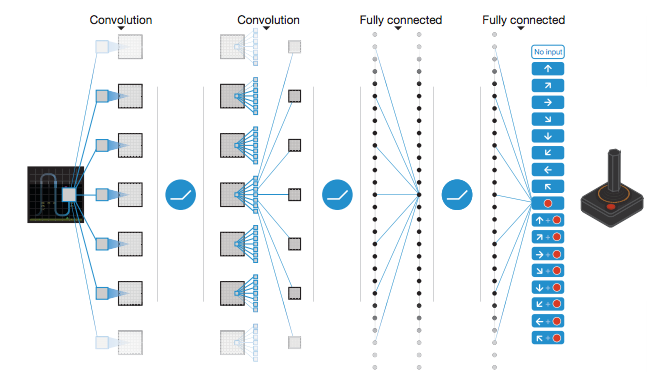
\includegraphics[width=6in]{../images/DQN}}

\slide{Watch The Video}

https://www.youtube.com/watch?v=V1eYniJ0Rnk

\slide{Asynchronous $Q$-Learning (Simplified)}
No replay buffer.
Many aynchronous threads each repeating:
\vfill

  \begin{quotation}
  \noindent $\tilde{\Theta} = \Theta$ (retrieve global $\Theta$)\newline \newline
  \noindent using policy $\argmax_a Q_{\tilde{\Theta}}(s,a)$ compute $$s_t,a_t,r_t,\ldots,s_{t+K},a_{t+K},r_{t+K}$$
  $$R_i = \sum_{\delta=0}^{t+K-i} \gamma^{i+\delta} r_{(i+\delta)}$$
  Update global $\Theta$:
  $$\Theta \;\minuseq\; \eta \sum_{i=t}^{t+K} \nabla_{\tilde{\Theta}}\;(Q_{\tilde{\Theta}}(s_i,a_i) - R_i)^2$$
  \end{quotation}

\slide{Policy Gradient}

We assume a parameterized policy $\pi_\Phi(a|s)$.

\vfill
$\pi_\Phi(a|s)$ is normalized while $Q_\Theta(s,a)$ is not.

\vfill
$$\Phi \;\pluseq\; \eta \nabla_\Phi \;R(\Phi)$$

\slide{Policy Gradient Theorem (Episodic Case)}
\begin{eqnarray*}
  \expect{R \;|\; \Phi} & = & \sum_{s_0,a_0,s_1,a_1,\ldots,s_T,a_T}\;\;P(s_0,a_0,s_1,a_1,\ldots,s_T,a_T)\;R \\
  \\
  \nabla_\Phi \;P(\ldots)R & = & P(S_0){\color{red} \nabla_\Phi \;\pi(a_0)}P(s_1)\pi(a_1) \cdots P(s_T)\pi(a_T)\;R \\
  & & + P(S_0)\pi(a_0)P(s_1){\color{red} \nabla_\Phi\;\pi(a_1)} \cdots P(s_T)\pi(a_T)\;R \\
  & & \vdots \\
  & & + P(S_0)\pi(a_0)P(s_1)\pi(a_1) \cdots P(s_T){\color{red} \nabla_\Phi\;\pi(a_T)}\;R \\
  \\
  & = & P(\ldots) \left(\sum_i\;\frac{\nabla_\Phi\;\pi_\Phi(a_i)}{\pi_\Phi(a_i)}\right) R
\end{eqnarray*}



\slide{Policy Gradient Theorem (Episodic Case)}
\begin{eqnarray*}
  \nabla_\Phi \;P(\ldots)R & = & P(S_0){\color{red} \nabla_\Phi \;\pi(a_0)}P(s_1)\pi(a_1) \cdots P(s_T)\pi(a_T)\;R \\
  & & + P(S_0)\pi(a_0)P(s_1){\color{red} \nabla_\Phi\;\pi(a_1)} \cdots P(s_T)\pi(a_T)\;R \\
  & & \vdots \\
  & & + P(S_0)\pi(a_0)P(s_1)\pi(a_1) \cdots P(s_T){\color{red} \nabla_\Phi\;\pi(a_T)}\;R \\
  \\
  & = & P(\ldots) \left(\sum_i\;\frac{\nabla_\Phi\;\pi_\Phi(a_i)}{\pi_\Phi(a_i)}\right) R \\
  \\
  \nabla_\Phi \;\expect{R \;|\; \Phi}& = & \expect{R \sum_t\;\nabla_\Phi\;\ln \pi_\Phi(a_t|s_t)}
\end{eqnarray*}

\slide{Policy Gradient Theorem}
\begin{eqnarray*}
 & &   \nabla_\Phi \;\expect{R \;|\; \Phi} \\
  \\
  & = & \expect{R \sum_t\;\nabla_\Phi\;\ln \pi_\Phi(a_t|s_t)} \\
  \\
  & = & E \sum_{t_1,t_2} r_{t_1} \nabla_\Phi\;\ln \pi_\Phi(a_{t_2}|s_{t_2}) \\
  \\
  & = & E \sum_{t_1 < t_2} r_{t_1} \nabla_\Phi\;\ln \pi_\Phi(a_{t_2}|s_{t_2})
  + E \sum_{t_1 \geq t_2} r_{t_1} \nabla_\Phi\;\ln \pi_\Phi(a_{t_1}|s_{t_2})
\end{eqnarray*}


\slide{Policy Gradient Theorem}
\begin{eqnarray*}
 & &   \nabla_\Phi \;\expect{R \;|\; \Phi} \\
  \\
    & = & {\color{red} E \sum_{t_1 < t_2} r_{t_1} \nabla_\Phi\;\ln \pi_\Phi(a_{t_2}|s_{t_2})}
  + E \sum_{t_1 \geq t_2} r_{t_1} \nabla_\Phi\;\ln \pi_\Phi(a_{t_1}|s_{t_2}) \\
  \\
  & = & \sum_{t_1 < t_2}\;E_{s_{t_1}}\;(E\; r_{t_1}|s_{t_1}) E_{s_{t_2}|s_{t_1}}\; \sum_{a_{t_2}} \pi_\Phi(a_{t_2}|s_{t_2})\nabla_\Phi\;\ln \pi_\Phi(a_{t_2}|s_{t_2}) + \cdots \\
  \\
  & & \sum_{t_1 < t_2}\;E_{s_{t_1}}\;(E\; r_{t_1}|s_{t_1}) E_{s_{t_2}|s_{t_1}}\; {\color{red} \sum_{a_{t_2}} \nabla_\Phi \;\pi_\Phi(a_{t_2}|s_{t_2}) \;\; = 0} 
\end{eqnarray*}

\slideplain{Policy Gradient Theorem}
\begin{eqnarray*}
  & &   \nabla_\Phi \;\expect{R \;|\; \Phi} \\
  \\
  & = & E \sum_{t_1 \leq t_2} \nabla_\Phi\;\ln \pi_\Phi(a_{t_1}|s_1) \;r_{t_2} \\
  \\
  & = & E\;\sum_t\; \nabla_\Phi\;\ln \pi_\Phi(a_t|s_t) \;R_{\geq t}
\end{eqnarray*}

\vfill
Sampling runs and computing the above sum over $t$ is Williams' REINFORCE algorithm.

\slide{Optimizing Discrete Decisions}

The REINFORCE algorithm is used generally for non-differentiable loss functions.

\vfill
For example error rate and BLEU score are non-differentiable --- they are defined on the result of discrete decisions.

\vfill

\slideplain{Policy Gradient Theorem}
\begin{eqnarray*}
  \nabla_\Phi \;\expect{R \;|\; \Phi} & = & E\;\sum_t\; \nabla_\Phi\; \ln \pi_\Phi(a_t|s_t) \;R_{\geq t} \\
  \\
  \\
  & = & \sum_s \rho(s) \sum_a \left(\nabla_\Phi \;\pi_\Phi(a|s)\right) Q^{\pi_\Phi}(s,a)
\end{eqnarray*}

\vfill
$\rho(s)$ is the expected number of occurances of $s$

\vfill
$Q^\pi(s,a) = \expectsub{\pi}{\sum_t\; r_t\;|\;s_0=s,\;a_0=a}$

\ignore{
\vfill
\eject

\centerline{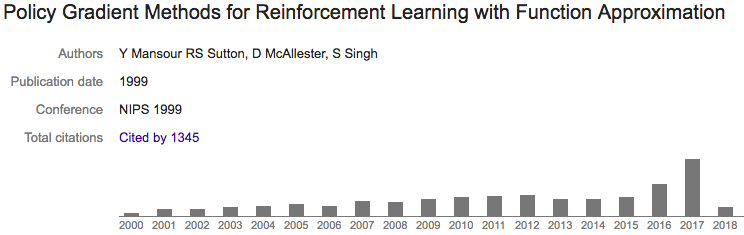
\includegraphics[width = 9.0in]{../images/Citations}}

\vfill
\centerline{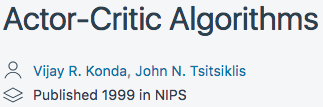
\includegraphics[width = 3.0in]{../images/Citations2}}
\centerline{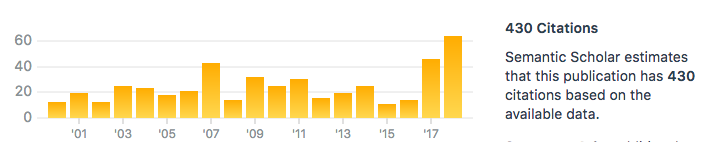
\includegraphics[width = 9.0in]{../images/Citations3}}
}

\slide{The Actor-Critic Algorithm}
\begin{eqnarray*}
  \nabla_\Phi \;\expect{R \;|\; \Phi} & = & E\;\sum_t\; \nabla_\Phi\; \ln \pi_\Phi(a_t|s_t) \;Q^{\pi_\Phi}(s_t,a_t) \\
  \\
  & \approx & E\;\sum_t\; \nabla_\Phi\; \ln \pi_\Phi(a_t|s_t) \;Q_\Psi(s_t,a_t) \\
\end{eqnarray*}

\vfill
We can reduce variance by using an estimator $Q_\Psi(s,a)$ for $Q^{\pi_\Phi}(s,a)$.

\vfill
$\pi_\Phi$ is the ``actor'' and $Q_\Psi$ is the ``critic''.

\slide{The Actor-Critic Algorithm}
\begin{eqnarray*}
  \nabla_\Phi \;\expect{R \;|\; \Phi} & \approx & E\;\sum_t\; \nabla_\Phi\; \ln \pi_\Phi(a_t|s_t) \;Q_\Psi(s_t,a_t) \\
\end{eqnarray*}

\begin{eqnarray*}
  \Phi  &\pluseq & \eta_1 \sum_t \left(\nabla_{\tilde{\Phi}}\;\ln \pi_{\tilde{\Phi}}(a_i|s_i)\right)Q_\Psi(s_t,a_t)\\
  \Psi & \minuseq & \eta_2 \sum_t \nabla_{\tilde{\Psi}}\;(Q_\Psi(s_t,a_t) - R_{\geq t})^2
\end{eqnarray*}

\vfill
$\pi_\Phi$ is the ``actor'' and $Q_\Psi$ is the ``critic''.

\slide{Advantage-Actor-Critic Theorem}

$$\nabla_\Phi R(\Phi) = \sum_s \rho(s) \sum_a \left(\nabla_\Phi\;\pi_\Phi(a|s)\right)(Q^{\pi_\Phi}(s,a) - V^{\pi_\Phi}(s))$$

\vfill
$V^\pi(s) = \expectsub{a \sim \pi(\cdot|s)}{Q(s,a)}$

\slide{}
\centerline{\bf Asynchronous Advantage Actor-Critic (A3C)}

\vfill
Asynchronous Methods for Deep Reinforcement Learning, Mnih et al., Arxiv, 2016 (Deep Mind)
\vfill
\vfill

\slide{Asynchronous Advantage Actor-Critic (A3C)}

\vfill
\begin{quotation}
  \noindent $\tilde{\Phi} = \Phi; \tilde{\Psi} = \Psi$ (retrieve global $\Phi$ and $\Psi$)\newline \newline
  \noindent using policy $\pi_{\tilde{\Phi}}$ compute $s_t,a_t,r_t,\ldots,s_{t+K},a_{t+K},r_{t+K}$
  $$R_i = \sum_{\delta=0}^{t+K-i} \gamma^{i+\delta} r_{(i+\delta)}$$
Update global $\Phi$ and $\Psi$
\begin{eqnarray*}
  \Phi  &\pluseq & \eta \sum_{i=t}^{t+K} \left(\nabla_{\tilde{\Phi}}\;\ln \pi_{\tilde{\Phi}}(a_i|s_i)\right)\left(R_i - V_{\tilde{\Psi}}(s_i)\right)\\
  \Psi & \minuseq & \eta \sum_{i=t}^{t+K} \nabla_{\tilde{\Psi}}\;(V_{\tilde{\Psi}}(s_i) - R_i)^2
  \end{eqnarray*}
\end{quotation}

\slide{Issue: Policies must be Exploratory}

The optimal policy is deterministic --- $a(s) = \argmax_a Q(s,a)$.

\vfill
However, a deterministic policy never samples alternative actions.

\vfill
Typically one forces a random action some small fraction of the time.


\slide{Issue: Discounted Reward}

DQN and A3C use discounted reward on episodic or long term problems.

\vfill
Presumably this is because actions have near term consequences.

\vfill
This should be properly handled in the mathematics.

\slide{Observation: Continuous Actions are Differentiable }

In problems like controlling an inverted pendulum, or robot control generally,
a continuous loss can be defined and the gradient of loss of with respect to a deterministic policy exists.

\slide{More Videos}

https://www.youtube.com/watch?v=g59nSURxYgk

https://www.youtube.com/watch?v=rAai4QzcYbs



\slide{END}

}
\end{document}


